\lhead{\emph{Results}}

% ***************************************************************************
\chapter{Results}
% ***************************************************************************

Each registration method is applied to estimate cameras relative positions on a recorded sequence containing 300s records for both kinect sensors. ICP method is applied in 3 different ways:

\begin{itemize}
    \item \emph{ICP} is the classical way of applying \acrshort{icp} for registration, we try to match one cloud with the other
    \item In \emph{ICP\_PointCloud} I apply the \acrshort{icp} for each point cloud to match with a given cloud of the complete scene. This cloud is a reconstruction previously prepared from both views, this techniques obviously requires a prior knowledge but it is good as a comparison with other methods. This point cloud contains objects on the table which may fail the \acrshort{icp} as it would try to match different shapes form the live point clouds.
    \item \emph{ICP\_CAD\_model} is the same method than the previous one but using a point cloud generated from a \acrshort{cad} model of the scene instead of a real reconstruction of the scene. This model doesn't contain any object that could help registration (especially the y translation).
\end{itemize}
Only the first method is satisfying our requirements for this work (no previous knowledge), the 2 others are applied for comparison purpose but assume that we have already solved the registration problem (reconstructed point cloud) or that we have a perfect knowledge of the expected result (\acrshort{cad}model). \\
Other methods are the ones explained in the previous sections:
\begin{itemize}
    \item \emph{plane\_matching}, registration using only plane matching, thus a $3^{rd}$ plane is added as explained in section \ref{sec:plane_detection}
    \item \emph{keypoints\_matching}, using only keypoint matching from section \ref{sec:3dkp}
    \item \emph{my\_method}, the method detailed in section \ref{chapt:implementation}, mixing both previous techniques.
\end{itemize}

\section{Distance and Angle Error}

From the estimated transform $\mathcal{T}_{1\,2}$ I extract translation vector ($t_x$, $t_y$, $t_z$) and Euler angles ($r_x$, $r_y$, $r_z$) as well as the 2 metrics explained in the previous section ($l$ and $\theta$). This 2 metrics give a easy overview of the transformation error in both translation and rotation in order to compare each method but the 6 other values will be used for a more detailed understanding of the errors.

\subsection{Real Scenario}

The combination of Keypoints and Planes matching makes the mixed method more effective to estimate translation than other methods (fig. \ref{fig:rot_comp})

\begin{figure}[h!]
    \centering
    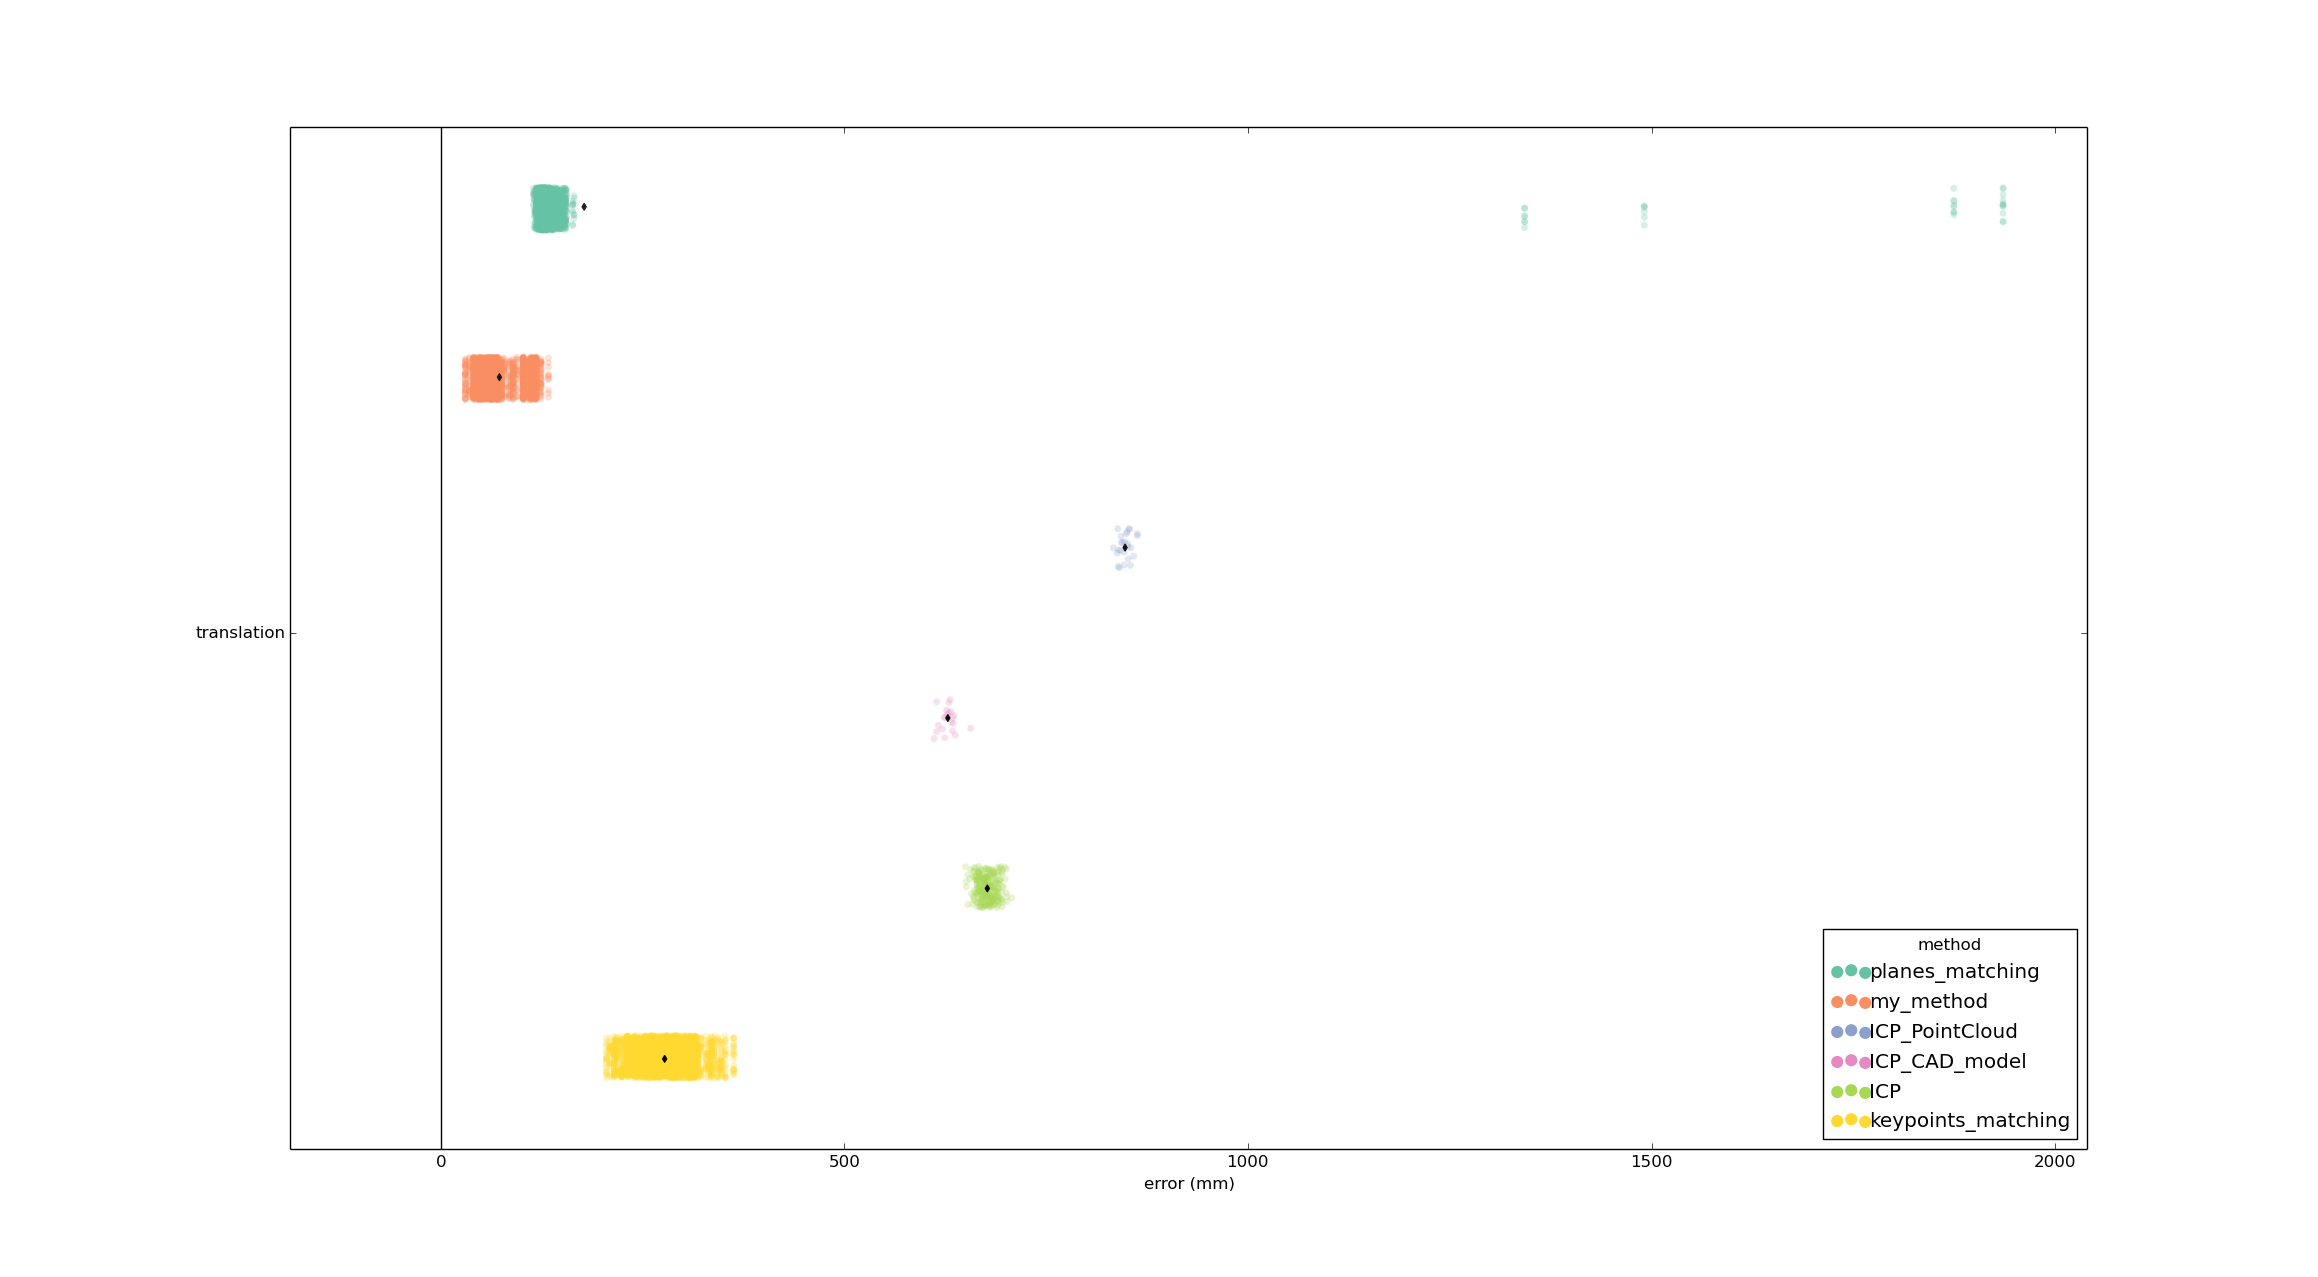
\includegraphics[width=\textwidth]{images/transl_comp.png}
    \caption{Comparison of translation error for each method.}
    \label{fig:trans_comp}
\end{figure}

The keypoints matching technique estimate almost as well the translation. In both cases the y-translation is obviously the one with the biggest error (and standard deviation) because of the symmetry in the scene along this axis.

\begin{figure}[h!]
    \centering
    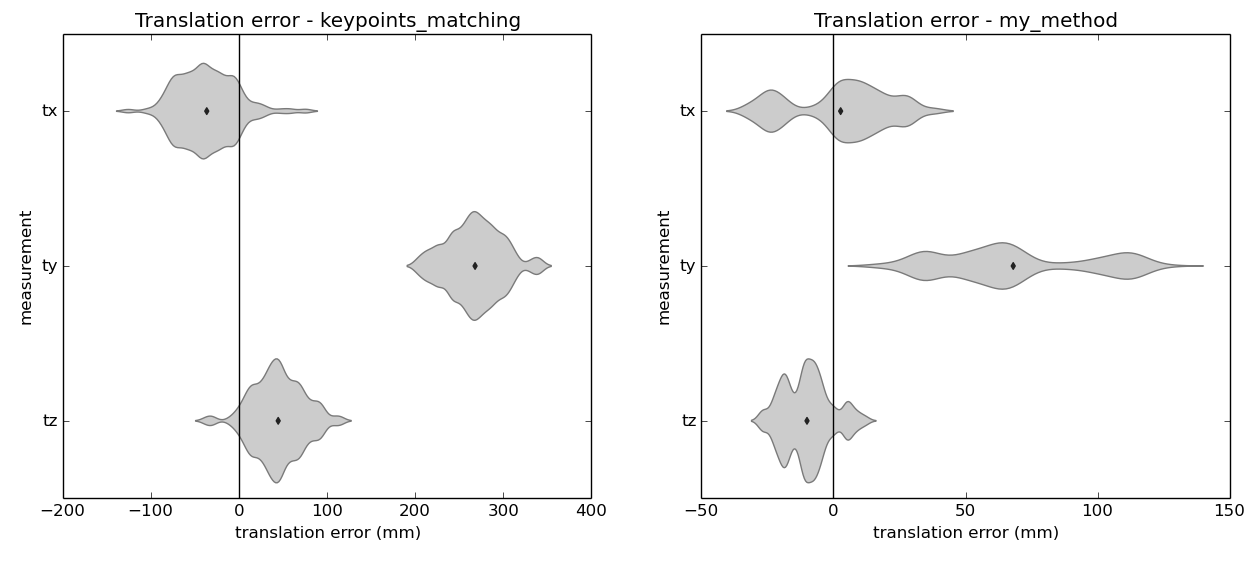
\includegraphics[width=\textwidth]{images/transl_violin.png}
    \caption{Translation error distribution.}
    \label{fig:transl_violin}
\end{figure}

To estimate the rotation, the best method is the plane alignment. Indeed, large planes provide a lot of distant points that reduce the angular error for the same. In the case of my method, the rotation error is increased because of keypoints alignment. This error can be reduced by using the projection of keypoints on plane intersection axis as described in \ref{}.

\begin{figure}[h!]
    \centering
    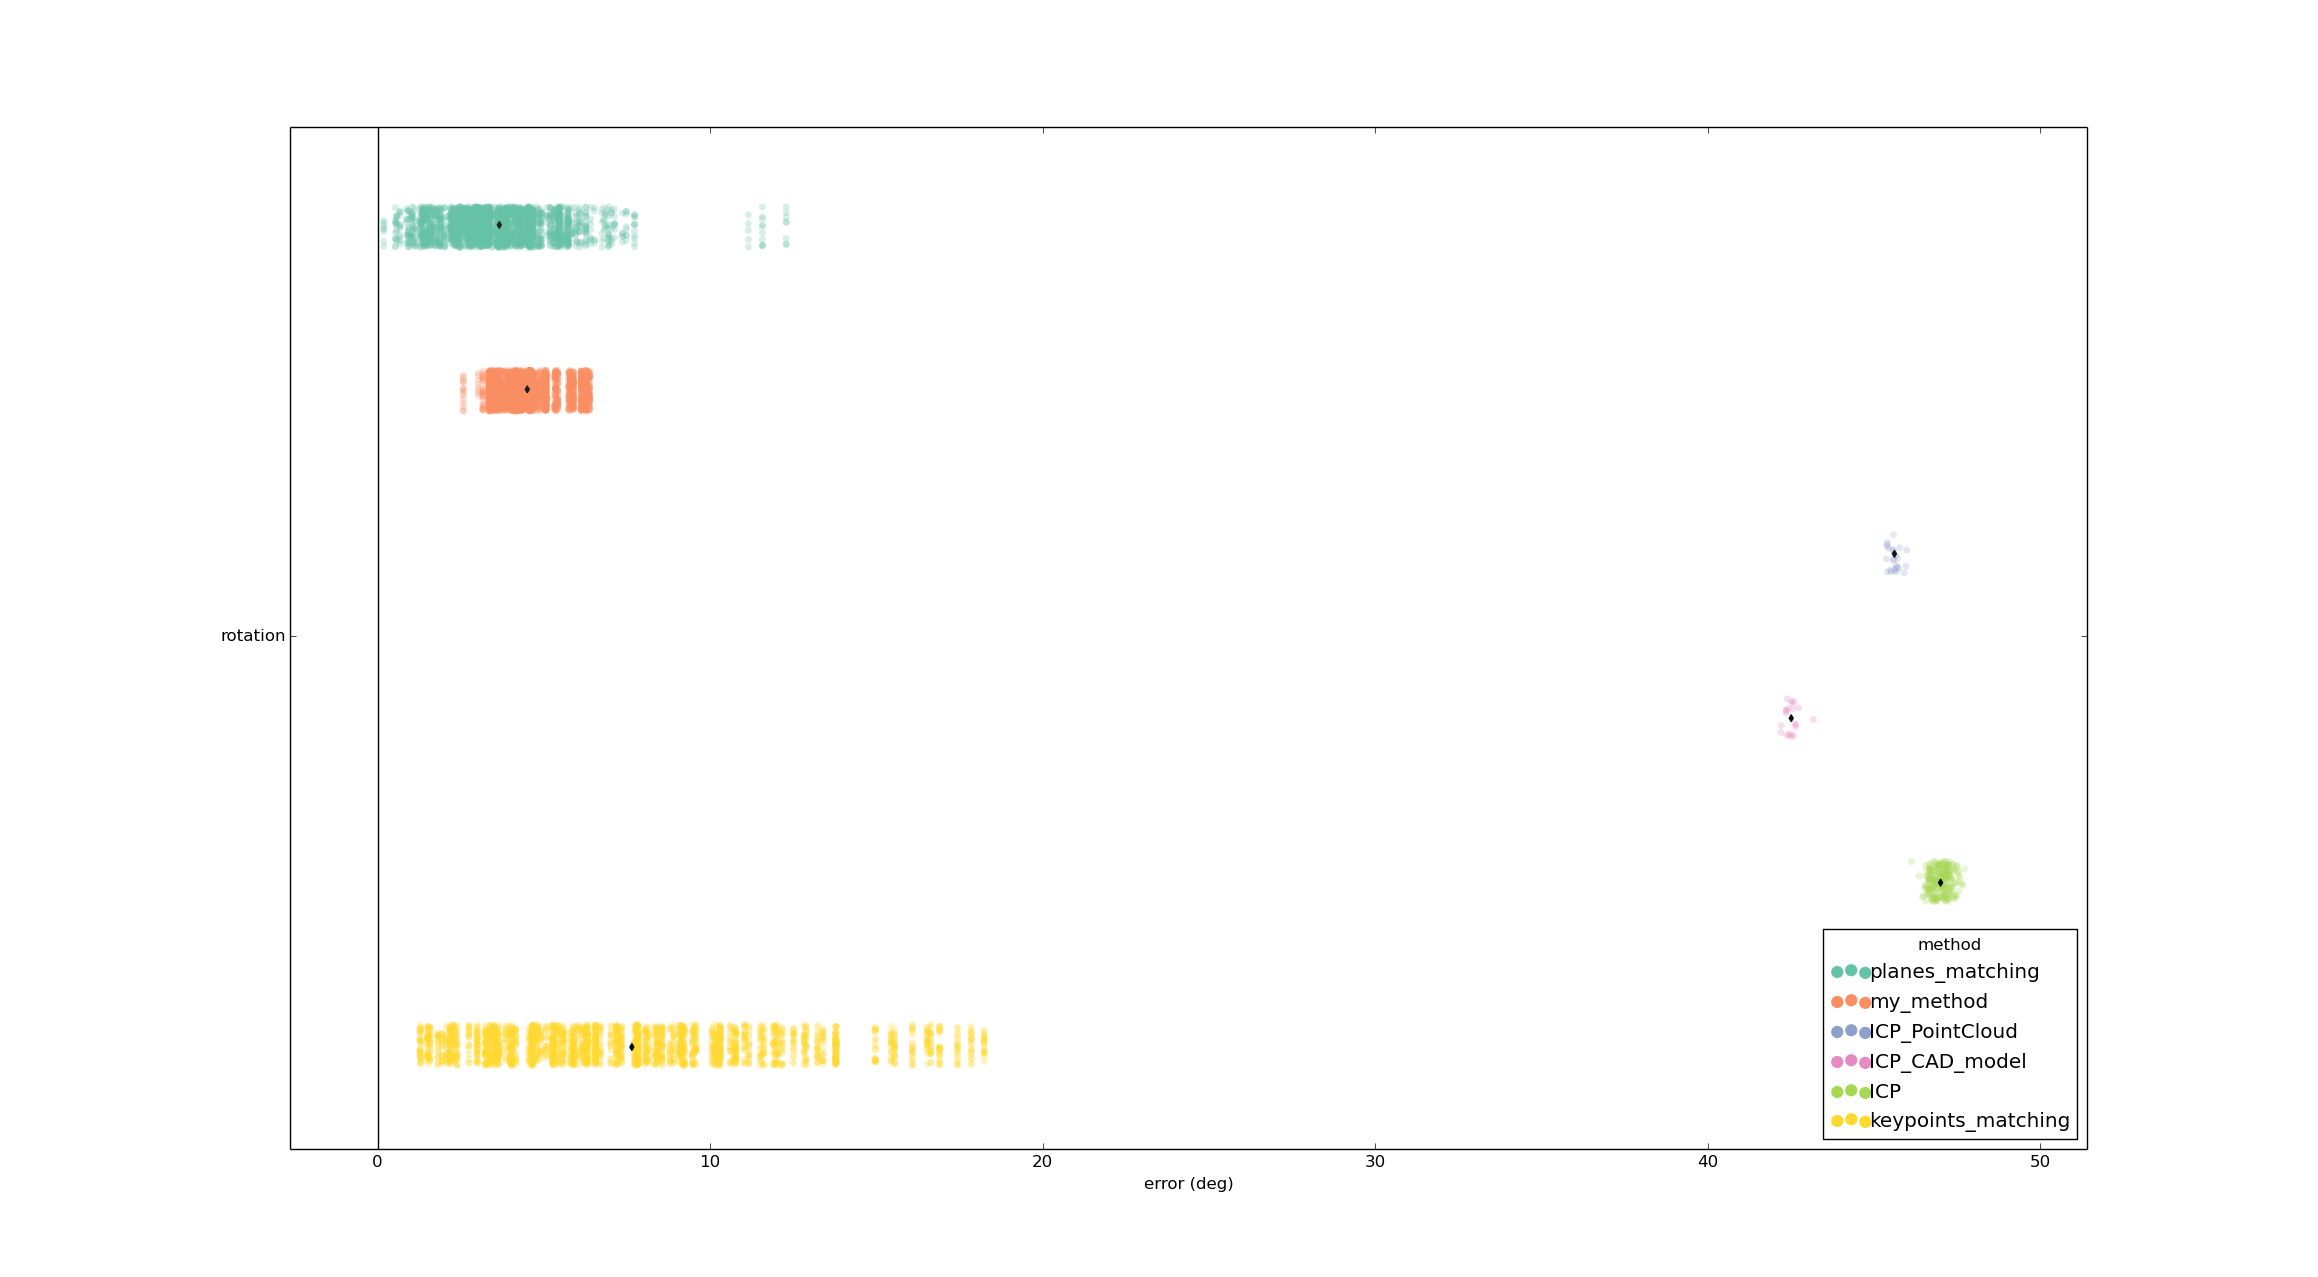
\includegraphics[width=\textwidth]{images/rot_comp.png}
    \caption{Comparison of rotation error for each method.}
    \label{fig:rot_comp}
\end{figure}

\begin{figure}[h!]
    \centering
    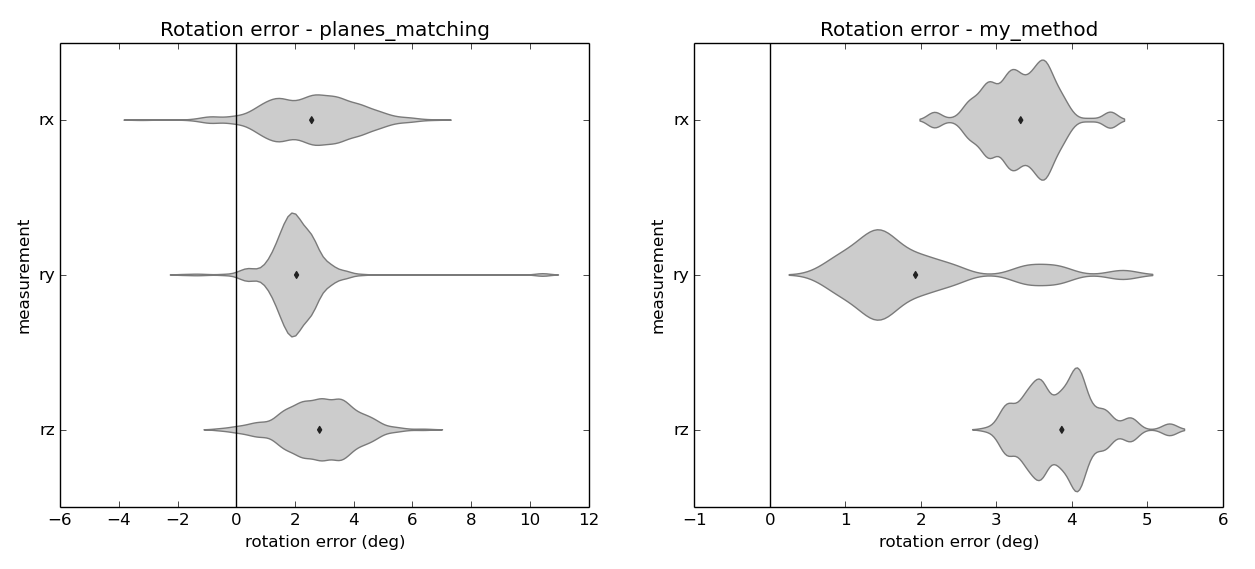
\includegraphics[width=\textwidth]{images/rot_violin.png}
    \caption{Rotation error distribution.}
    \label{fig:rot_violin}
\end{figure}

\section{Computing Speed}